\documentclass[tikz]{standalone}
\usepackage{tikz}
\usepackage{tikz}
\usetikzlibrary{shapes}
\tikzstyle{mir}=[double]
\tikzstyle{d2}=[diamond,aspect=2,scale=0.5,draw]
\tikzstyle{d4}=[diamond,scale=0.5,rotate=45,draw]
\tikzstyle{d6}=[regular polygon, regular polygon sides=6,scale=0.5,draw]

\begin{document}
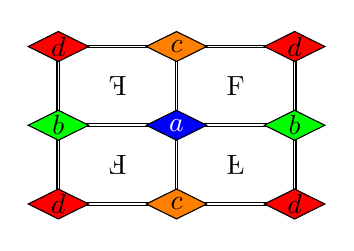
\begin{tikzpicture}
\draw (-1.5, 0)--(1.5, 0) [mir];
\draw (-1.5, -1)--(1.5, -1) [mir];
\draw (-1.5, 1)--(1.5, 1) [mir];
\draw (-1.5, -1)--(-1.5, 1) [mir];
\draw (0, -1)--(0, 1) [mir];
\draw (1.5, -1)--(1.5, 1) [mir];

\draw (0, 0) node [d2, scale=2.2, fill=blue] {};
\draw (0, 0) node [color=white] {$a$};

\draw (-1.5, 0) node [d2, scale=2.2, fill=green] {};
\draw (-1.5, 0) node {$b$};
\draw (1.5, 0) node [d2, scale=2.2, fill=green] {};
\draw (1.5, 0) node {$b$};

\draw (0, -1) node [d2, scale=2.2, fill=orange] {};
\draw (0, -1) node {$c$};
\draw (0, 1) node [d2, scale=2.2, fill=orange] {};
\draw (0, 1) node {$c$};

\draw (-1.5, -1) node [d2, scale=2.2, fill=red] {};
\draw (-1.5, -1) node {$d$};
\draw (1.5, -1) node [d2, scale=2.2, fill=red] {};
\draw (1.5, -1) node {$d$};
\draw (-1.5, 1) node [d2, scale=2.2, fill=red] {};
\draw (-1.5, 1) node {$d$};
\draw (1.5, 1) node [d2, scale=2.2, fill=red] {};
\draw (1.5, 1) node {$d$};

\draw (.75, .5) node {F};
\draw (-.75, .5) node [xscale=-1] {F};
\draw (.75, -.5) node [yscale=-1] {F};
\draw (-.75, -.5) node [rotate=180] {F};

\end{tikzpicture}
\end{document}
